\chapter{Base Manipulation of Symmetric-tip Needles} \label{chap:chap-3}

\section{Chapter Overview}
\label{sec:chap-3-overview}

This chapter expands upon previous discussion of needle base manipulation, and extends the preliminary model presented in~\cref{chap:chap-2}. Specifically, we present a needle-tissue interaction model that takes into account multilayered, nonlinear soft tissue environment during needle insertion, and a simulation environment that resolves such model at interactive rate. Using fiber Bragg grating optical strain feedback at sparse location along the needle, needle shape can be reconstructed in realtime. We also explore the use of resolved-rate control for symmetric-tip needle base manipulation, and presents a series of tissue phantom experiments to validate our approach.

% \begin{itemize}
% \item Model: RAL 2023
% \item Control: ISMR 2023
% \item Feedback: TMRB 2024
% \end{itemize}

\section{Modeling of Needle Base Manipulation}
\label{sec:chap-3-model}

During \textit{in situ} needle bending for spinal injections, part of the flexible needle is already inserted into the soft skin and muscle tissues, and needle manipulation is applied at the needle base. A schematic of the physical scenario is shown in~\cref{fig:chap-3-model-schematic}.

\begin{figure}[t]
  \centering
  \includegraphics[width = \columnwidth]{figures/base_manipulation/1/model_schematic.png}
  \caption{Schematic of needle interaction with a multilayer medium. Motion applied to the needle base is represented as boundary conditions. Tissue response will differ with different tissue properties. Slope at the needle base forms a needle RCM, while actual needle COM deviates from the RCM due to inherent flexibility of the needle as well as reaction forces generated by the tissue.}
  \label{fig:chap-3-model-schematic}
\end{figure}

\subsection{Needle-Tissue Interaction Model}
\label{sec:chap-3-needle-tissue-interaction-model}

The proposed interaction model resembles closely to an Euler-Bernoulli beam with flexible support.  The needle, modeled as a homogeneous beam, is initially at rest along the horizontal $x-$axis and embedded in a multilayer medium, with inserted depth $l$. Boundary conditions are applied to the needle base such that it is displaced in by $d_b$, and tilted by a slope $k_b$. The control distance, $s_b$, separates the point of application of boundary conditions from the point of needle insertion. Due to the flexibility of the needle and the contact with soft tissue, the needle will deform upon base motion, assuming a shape $u(x)$, and the corresponding force generated within the medium is $F(x) = \sum f_i(x)$. If the medium presents no resistance to the needle, i.e. $F = 0$, the needle would remain straight and intersect the $x-$axis at an RCM; however, reactive force from the medium will bend the needle, causing it to intersect the $x-$axis elsewhere, called the needle COM.

\begin{figure}[t]
  \centering
  \includegraphics[width = \columnwidth]{figures/base_manipulation/1/experiment_setup.png}
  \caption{Experiment setup to study \textit{in situ} needle bending. The active linear stage and passive rotary stage generate needle base motion. Markers on the stage and container are detectable in CT scans, and are used to calculate needle base motion from relative frame transformations.}
  \label{fig:chap-3-experiment-setup}
\end{figure}

The reaction force from each medium, $f_i(x)$, will be proportional to the degree of tissue compression. Many have treated the proportionality as a constant, $k$, which can be regarded as a hyperparameter and the tissue is modeled as a ``virtual spring'' with a constant coefficient~\parencite{glozmanImageGuidedRoboticFlexible2007}. However, biological soft tissues, such as skin and skeletal muscles, exhibit complex nonlinear stretch-stress behavior, which cannot be characterized effectively using a constant spring model~\parencite{humphreyIntroductionBiomechanicsSolids2025}.

In order to account for the nonlinear behavior of the tissue, we treat the proportionality function $k(x)$ as the tangent modulus of the material, i.e.
\begin{equation}
  \label{eq:chap-3-tangent-modulus}
  k(x) = \frac{\partial S}{\partial \lambda_c}
\end{equation}
where $\lambda_c$ is the compression ratio, and $S$ is the expression for engineering stress $(P)$ or true stress $(\sigma)$:
\begin{align}
  P &= \sum_{i = 1}^3\left(\frac{\partial W}{\partial \lambda_i} - \rho \lambda_i^{-1}\right)\textbf{v}^{(i)} \otimes \textbf{u}^{(i)},    \label{eq:chap-3-engineering-stress} \\
    \sigma & = \sum_{i = 1}^3\left(\lambda_i \frac{\partial W}{\partial \lambda_i} - \rho\right)\textbf{v}^{(i)} \otimes \textbf{v}^{(i)}.   \label{eq:chap-3-true-stress}
\end{align}

The function $W$ in~\cref{eq:chap-3-engineering-stress,eq:chap-3-true-stress} is the strain energy function of an incompressible hyperelastic material, and $\lambda_i$ is the stretch ratio of the tissue in the $i$-th principal direction. Variable $\rho$ is a Lagrangian multiplier that ensures material incompressibility, and vectors $\textbf{u}^{(i)}$ and $\textbf{v}^{(i)}$ are the $i$-th eigenvector of the right- and left-stretch tensors, respectively.

Since the tissue can only be compressed in the direction of needle displacement,
\begin{equation}
  \label{eq:chap-3-compression}
  \lambda_c = \frac{t_{0} - |u(x)|}{t_{0}},
\end{equation}
where $t_{0}$ is the initial length of the tissue, so that $\lambda_c \leq 1$ in the direction of compression. Referring to~\cref{fig:chap-3-model-schematic}, the assigned direction of compression is along the $y-$axis, i.e. $\lambda_c = \lambda_2$.

An assumption made for multilayer insertion scenarios is that when the needle slope is locally small, compression happens mostly in the $y-$direction such that layer boundaries remain in place, i.e. the tissue is constrained within its own ``compartment'' and does not expand in the direction of layer boundaries~\parencite{glozmanImageGuidedRoboticFlexible2007}. Such an assumption will be tested with experiment. Here, without specifying the choice of hyperelastic material model $W$ and stress model $S$, we leave the expression of $f_i(x)$ as
\begin{align}
  \label{eq:chap-3-fx-general}
  \begin{split}
    f_i(x) &= k_i(x)u(x)\left\{ 1 - \gamma_i\sin^2\left[ \tan^{-1}\left( u_{,x}(x) \right) \right] \right\}, \\
           & x \in [x_{il}, x_{ir}].
  \end{split}
\end{align}
defined within the layer boundaries $x_{il}$ and $x_{ir}$. The constant $\gamma_i$ is the friction coefficient between the needle and the medium, and the term in curly brackets accounts for the friction that must happen to keep the needle tip at the same depth during needle motion. Since locally the needle slope is small, and biological soft tissues have high water content, $f_i(x)\approx k_i(x)u(x)$ when $\gamma_i \ll 1$.

Using comma to denote derivative, the strong form of the problem is as follows: given constants $d_b$ and $k_b$, and function $F(x)$, find $u(x) \in C^4\left(-s_b, l\right)$ such that
\begin{align}
  \label{eq:chap-3-complete-formulation}
  \begin{split}
    EIu,_{xxxx} &= F(x) \quad x\in \left(-s_b, l\right), \\
    u(-s_b) &= d_b, \quad u,_{x}(-s_b) = k_b, \\
    u,_{xx}(l) &= 0, \quad u,_{xxx}(l) = 0.     
  \end{split}
\end{align}

\subsection{Material Model Selection and Characterization}
\label{sec:chap-3-material-model-selection-and-characterization}

Liquid plastisols, commonly used in medical robotics research as an ingredient for making tissue phantoms, are used as a test material for choosing a proper material model and obtaining relevant model parameters. Incompressible hyperelastic material models are adopted based on their success in describing rubber-like materials and biological soft tissues. Common models include Neo-Hookean, Mooney-Rivlin, Yeoh, and Ogden~\parencite{martinsComparativeStudySeveral2006,singhMechanicalPropertiesWholebody2021,heComparativeStudy852022}.

In order to choose a hyperelastic material model and to obtain parameter values for the tissue phantom, cylindrical samples are fabricated from liquid plastisol (142 Super Soft, Bait Plastics, MO, USA) and tested with an electromechanical test system (MTS, Minnesota, USA). Unconfined compression tests are carried out as suggested by the ASTM standard for compression up to 5N~\parencite{StandardTestMethods}. The equipment and method used to fabricate test samples are introduced in appendix~\ref{chap:appendix-a}.

Since the sample's cross-sectional area cannot be measured accurately during the compression test, only the engineering stress can be calculated, therefore an unconstrained compression model with engineering stress (denoted as \textit{UEng}) is deemed appropriate for the PVC material, and will be used in~\cref{eq:chap-3-tangent-modulus}.

For biological soft tissues, it has been reported that porcine skeletal muscles resemble closely to human skeletal muscles in terms of their mechanical behaviors~\parencite{moVitroCompressiveProperties2020}, which can be captured reasonably well with a one-term Ogden hyperelastic model. Both an unconstrained true stress model (\textit{UTru}) and a constrained true stress model (\textit{CTru}) will be used in~\cref{eq:chap-3-tangent-modulus}.

\subsection{Experiment Setup and Design}
\label{sec:chap-3-experiment-setup-and-design-1}

A setup to replicate \textit{in situ} needle bending and to verify the proposed interaction model is shown in~\cref{fig:chap-3-experiment-setup}. The needle base maneuver can be decomposed into a lateral translation and a local rotation, as denoted by $d_b$ and $k_b$ in~\cref{fig:chap-3-model-schematic} and~\cref{eq:chap-3-complete-formulation}.

As shown in~\cref{fig:chap-3-motion-schematic}, the active linear stage will apply a lateral translation, and the passive rotary stage will rotate freely such that the needle will assume a least-energy configuration, forming a slope $k_b$ at the needle base. Since the point of needle base rotation is further away from the entry point than the control distance, the actual magnitude of $d_b$ will be less than the amount of linear stage translation.

A stainless steel trocar needle of 1mm diameter is used in the experiment. Single layer of PVC tissue phantoms and porcine skeletal muscle samples are used as the surrounding medium. For the PVC phantoms, material models and parameters are obtained from compression tests, while the material properties for the porcine skeletal muscles are retrieved from literature, as described in~\cref{sec:chap-3-material-model-selection-and-characterization}.

\begin{figure}[t]
  \centering
  \includegraphics[width = 0.68\columnwidth]{figures/base_manipulation/1/motion_schematic.png}
  \caption{A top-down view of the needle base motion. When a lateral translation is applied, the inserted needle will bend and rotate freely about the passive rotary stage. The needle is allowed to freely translate in the axial direction so that the needle tip remains at the same insertion depth.}
  \label{fig:chap-3-motion-schematic}
\end{figure}

Three inserted depths of the needle $l \in [20, 40, 60]$ mm, as well as two control distances $s_b \in [20, 40]$ mm, are chosen as initial configurations. The linear stage translates laterally from -15 mm to +15 mm with 2.5 mm increments. In sum, 156 data points are included in the experiment for the PVC tissue phantoms and porcine skeletal muscle samples.

Any metallic object will appear as an artifact in MRI images, therefore the needle shape cannot be determined precisely. In order to validate the proposed model, ground truth needle shapes will be extracted from CT images; motion parameters, $d_b$ and $k_b$, can also be obtained from successive CT scans.

\subsubsection{Image Registration and Segmentation}
\label{sec:chap-3-image-reg-and-seg}
Steel markers of two different sizes are embedded on the needle stage ($stg$) and the acrylic container ($ctn$), so as to differentiate between the moving stage frame $F_{stg}$ and the fixed container frame $F_{ctn}$. The needle and markers can be detected by the CT scanner (Loop-X, BrainLab, Munich, Germany) and segmented with intensity thresholding.

In order to extract needle base motion and other model parameters, a baseline scan is first taken to ensure the insertion is straight and perpendicular to the top surface of the medium. Control distance $s_b$ and inserted depth $l$, as well as the baseline stage frame $F_{stg0}$ is obtained from the baseline volume. The needle tip position is determined by the last detectable needle voxel after intensity thresholding. Subsequent volumes use the fixed container frame as global reference, and needle base motion, $d_b$ and $k_b$, can be extracted from relative frame changes between $F_{stgi}$ and $F_{stg0}$.

An iterative closest point (ICP) method is used to register the markers detected in CT, $F^{CT}$, with their positions by design, $F^{DN}$. A brief explanation for finding relative needle base motions is offered in~\cref{alg:base_motion_CT}.

A total of seven markers are placed on the moving stage, and twelve on the fixed container. Since only a few number of markers are used, and the components are fabricated with high accuracy, a one-to-one mapping between detected and designed marker positions is possible. A wrapper around the ICP algorithm performs random rotations to the point clouds until such mapping is established. In the rare cases where a marker moved outside of the volume, point rejection is performed to ensure equally accurate mapping on the remaining markers.

\begin{algorithm}
  \caption{Needle base motion from CT}
  \label{alg:base_motion_CT}
  \begin{algorithmic}[1]
    \State $[needle, cntCT, stgCT] \gets seg(CT)$  \Comment{segment needle, container and stage markers from CT}
    \State $F_{cnt}^{CT \to DN} \gets ICP(ctnDN, ctnCT)$ \Comment{map container CT to design (\textit{DN})}
    \State $stgCT' \gets FrameTransform(F_{cnt}^{DN \to CT}, stgCT)$ \Comment{transform stage CT with $F_{cnt}^{CT \to DN}$}
    \State $F_{stg}^{DN \to CT} \gets ICP(stgCT', stgDN)$ \Comment{map stage design to CT}
    \State $[R, t] \gets$ Extract needle base rotation and translation from $F_{stg}^{DN \to CT}$
    \State $d_b \gets t[2] - t_0[2]$
    \State $k_b \gets \tan(\atantwo(R[2, 1], R[1, 1)])$ \Comment{using ZYX Euler angles, extracting only Z component}
  \end{algorithmic}
\end{algorithm}

\subsubsection{Mechanical Testing and Model Selection}
\label{sec:chap-3-mechanical-testing-and-model-selection}

The stretch-stress curves from compression tests are fitted with different hyperelastic models. For computational efficiency, two parameters are kept for curve fitting for models that have variable number of terms and parameters. As shown in~\cref{fig:hyperelastic_model_fitting}, candidate hyperelastic models: one-term Ogden, one-term Mooney-Rivlin, two-term Yeoh, and Neo-Hookean all fit the material well, with $R^2 > 99\%$; however, the Neo-Hookean model deviates from the other models when the compression ratio is higher than 0.8, therefore the Neo-Hookean model is rejected for inconsistency with the other models. The one-term Ogden model is selected for the PVC material, while the other two are equally valid choices.

\begin{figure}[t]
  \centering
  \includegraphics[width = 0.65\columnwidth]{manuscripts/RAL_2023//figures/compression_tests.png}
  \caption{Hyperelastic model fitting with selected number of specimens that showed consistent stretch-stress behaviors. All four models produce good fits, but the Neo-Hookean model deviates from the rest in compression higher than 0.8.}
  \label{fig:hyperelastic_model_fitting}
\end{figure}

The one-term Ogden model with incompressibility constraint has form
\begin{equation}
  \label{eq:incompressible_ogden}
  W = \frac{2\mu}{\alpha^2}(\lambda_1^{\alpha} + \lambda_2^{\alpha} + \lambda_3^{\alpha} - 3) - \rho (J - 1),
\end{equation}
where $\mu$ is the material shear modulus, and $\alpha$ is a model parameter that determines the overall shape of the stretch-stress curve. Constant $J = \det{\mathbf{F}}$, where $\mathbf{F}$ is the deformation gradient that is dependent on the choice of compression model, i.e. unconstrained ($\mathbf{F = F_U}$) or constrained ($\mathbf{F = F_C}$). For $\mathbf{F = F_C}$, the tissue is restricted from expanding along the $x-$ direction, i.e. $\lambda_1=1$.
\begin{align}
  \mathbf{F_U} &= \diag{\left( \lambda_1, \lambda_2, \lambda_3 \right)} = \diag{\left(\frac{1}{\sqrt{\lambda_c}}, \lambda_c, \frac{1}{\sqrt{\lambda_c}} \right)},
                 \label{eq:unconstrained_deformation_gradient} \\
  \mathbf{F_C} &= \diag{\left( \lambda_1, \lambda_2, \lambda_3 \right)} = \diag{\left( 1, \lambda_c, \frac{1}{\lambda_c}\right)}.
                 \label{eq:constrained_deformation_gradient}
\end{align}

Model parameters for this PVC phantom are $\mu = 12.72$ kPa, and $\alpha = -1$. Due to the nature of the compression test, the \textit{UEng} model will be assigned to the PVC material.

Fresh pork loin are used as porcine skeletal muscle samples in \textit{ex vivo} experiments. According to~\parencite{moVitroCompressiveProperties2020}, model parameters for porcine skeletal muscles are $\mu = 3.63$ kPa and $\alpha = 8.74$. For the porcine sample, both \textit{UTru} and \textit{CTru} compression models are used in the simulation.

\subsubsection{Image Registration and Needle Reconstruction}
\label{sec:chap-3-image-reg-and-needle-recon}

\begin{figure}[t]
  \centering
  \includegraphics[width = \columnwidth]{manuscripts/RAL_2023/figures/multilayer_demo.png}
  \caption{FEM simulation of \textit{in situ} needle bending of an initially straight needle embedded in a multilayer medium with increasing stiffness. Lateral displacement of 15mm and slope of $-40\%$ are applied at the needle base. Slope at the needle base results in an RCM at $x = 17.5$mm, while the needle COM is located at $x = 40.0$mm.}
  \label{fig:chap-3-multilayer-demo}
\end{figure}

The CT scanner uses an adaptive image acquisition method that produces variable slice spacing for different scans. The average slice spacing is approximately 0.5 mm.

Using the centroids of detected markers volumes as their physical positions, the mean image registration error is 0.1 mm for the stage markers, and 0.2 mm for the container markers, due to slightly less accurate construction method of the acrylic container. The needle shape is reconstructed by a linear interpolation of the centroids of detected needle volume. Since the interpolation is performed voxel-wise, the interpolated shape truthfully represents the shape detected by the scanner, and no slope information is injected into the detected needle shape.

\subsection{Simulation and Experiment Results}
\label{sec:chap-3-simulation-and-experiment-results}

\begin{figure}[tb]
  \centering
  \includegraphics[width = \textwidth]{manuscripts/RAL_2023/figures/simulation_vs_experiment.png}
  \caption{Detected needle shape overlaid with simulated needle shape on a porcine sample by the \textit{UTru} model. Point of insertion is at the origin. For a 60mm inserted depth and 40mm control distance, the least-energy needle RCM lands at approximately 23mm underneath the entry point, while the actual needle COM is at around 38mm. The simulated COM falls short at around 33mm.}
  \label{fig:chap-3-simulation-vs-experiment}
\end{figure}

A custom FEM routine is written in MATLAB to solve the boundary value problem proposed in~\cref{eq:chap-3-complete-formulation}. The needle is discretized into 1 mm elements, and piecewise cubic Hermite interpolating polynomials and two-node isoparametric elements are used. Although only single-layer materials are used in the current experiment, the FEM routine is capable of simulating multilayer scenarios, as shown in~\cref{fig:chap-3-multilayer-demo}.

The stainless steel needle is assigned a Young's Modulus of 200 GPa. Bent needle shapes detected by the CT scanner are compared against simulated shapes, provided the extracted needle base motions as well as material model parameters. Result of a typical trial is shown in~\cref{fig:chap-3-simulation-vs-experiment}, with the reconstructed shapes overlaid with  simulated shapes, as well as detected needle RCM, COM, and simulated COM as a result of needle motion.

A total of 156 CT scans are taken and analyzed. \Cref{tab:rcm_vs_com} lists the depths of needle RCM and COM with different combinations of inserted depths of the needle, materials and control distances.

Comparing by inserted depths $l$, when the $l$ is small, the RCM and COM are located close to each other; but as $l$ increases, so does the difference between the two centers. The depths of RCM and COM for porcine skeletal muscle sample (PSM, $\mu = 3.63$ kPa) increase steadily with increasing $l$, while the RCM for PVC ($\mu = 12.72$ kPa) becomes shallower when the control distance $s_b$ increases, indicating that the needle bends more outside of the tissue than the cases where the control distance is shorter.

In all cases, the natural RCM formed by the needle are not at the needle insertion point; their locations are instead dependent on the local relative stiffness of the needle and its surroundings. The needle COM has a more predictable and consistent behavior, at which point the net tissue displacement is zero, acting as an actual pivot point of the flexible needle.

\begin{table}[t]
\centering
\caption{Detected and Simulated Needle RCM, COM [mm]}
\begin{tabular}{c|ccc|ccc|c}
\cline{1-7}
\multicolumn{1}{|c|}{\diagbox{M}{$l$}} & \multicolumn{1}{c|}{20} & \multicolumn{1}{c|}{40} & 60 & \multicolumn{1}{c|}{20} & \multicolumn{1}{c|}{40} & 60 &  \\ \hline
\multicolumn{1}{|c|}{} & \multicolumn{1}{c|}{9.7} & \multicolumn{1}{c|}{10.9} & 9.0 & \multicolumn{1}{c|}{8.4} & \multicolumn{1}{c|}{6.8} & 2.6 & \multicolumn{1}{c|}{RCM} \\ \cline{2-8} 
\multicolumn{1}{|c|}{PVC} & \multicolumn{1}{c|}{10.3} & \multicolumn{1}{c|}{24.3} & 31.1 & \multicolumn{1}{c|}{10.9} & \multicolumn{1}{c|}{23.9} & 37.5 & \multicolumn{1}{c|}{COM} \\ \cline{2-8} 
\multicolumn{1}{|c|}{} & \multicolumn{1}{c|}{11.3} & \multicolumn{1}{c|}{21.3} & 25.9 & \multicolumn{1}{c|}{11.4} & \multicolumn{1}{c|}{21.0} & 25.5 & \multicolumn{1}{c|}{COM$_{sim}$} \\ \hline
\multicolumn{1}{|c|}{} & \multicolumn{1}{c|}{12.6} & \multicolumn{1}{c|}{21.0} & 26.2 & \multicolumn{1}{c|}{11.9} & \multicolumn{1}{c|}{20.6} & 22.6 & \multicolumn{1}{c|}{RCM} \\ \cline{2-8} 
\multicolumn{1}{|c|}{PSM} & \multicolumn{1}{c|}{13.4} & \multicolumn{1}{c|}{25.7} & 39.5 & \multicolumn{1}{c|}{10.6} & \multicolumn{1}{c|}{25.7} & 38.5 & \multicolumn{1}{c|}{COM} \\ \cline{2-8} 
\multicolumn{1}{|c|}{} & \multicolumn{1}{c|}{12.7} & \multicolumn{1}{c|}{23.8} & 35.0 & \multicolumn{1}{c|}{11.8} & \multicolumn{1}{c|}{23.1} & 33.8 & \multicolumn{1}{c|}{COM$_{sim}$} \\ \hline
 & \multicolumn{3}{c|}{20} & \multicolumn{3}{c|}{40} & \multicolumn{1}{c|}{sb} \\ \cline{2-8} 
\end{tabular}
  \label{tab:rcm_vs_com}
\end{table}

\subsubsection{Error Analysis}
\label{sec:chap-3-error-analysis}

 \begin{figure}[t]
   \centering
   \includegraphics[width = \columnwidth]{manuscripts/RAL_2023/figures/error_heatmaps.png}
   \caption{Median and maximum needle tip position simulation errors as compared with detected positions from CT. Unit in millimeters.}
   \label{fig:chap-3-error-heatmaps}
\end{figure}


The needle tip prediction errors, calculated as the absolute distance between the detected and simulated needle tip, are shown as heatmaps in~\cref{fig:chap-3-error-heatmaps}. The effects of choice of compression models (\textit{UEng, UTru, CTru}) and parameter values are explored. In terms of parameter values, subscript \textit{C} indicates that the correct values are assigned to the corresponding material, while subscript \textit{I} indicates that the incorrect values from the other material are used for the current material.

As shown in the figure, when proper material parameters and compression models are used, the errors on average can be kept at around 0.2 mm for all inserted depths. In particular, prediction for porcine skeletal muscles with the \textit{UTru} compression model has a maximum error of less than 0.5mm and median error less than 0.2mm, producing better overall tip position prediction than the other two models.

When taking the inserted depths $l$ into account, it is evident from Figure~\ref{fig:chap-3-error-boxplots} that at a shallow depth, the influence of compression models and material properties is limited, since the needle will bend less and the higher stiffness of the needle decides the overall behavior; however, this is not the case when the inserted depth is large, for which the effect of tissue compression is non-negligible. The \textit{UTru} model for porcine skeletal muscle samples produces more consistent results overall, achieving a mean error of 0.15 mm with variance 0.01 mm$^2$.

\begin{figure}[t]
   \centering
   \includegraphics[width = \columnwidth]{manuscripts/RAL_2023/figures/error_boxplots.png}
   \caption{Simulation error distribution of porcine samples at different depths and with different compression models as well as parameter values. Unit in millimeters.}
   \label{fig:chap-3-error-boxplots}
 \end{figure}

\subsection{Clinical Relevance}
\label{sec:clinical_relevance}

The proposed needle-tissue interaction model helps establish the groundwork for needle shape prediction during \textit{in situ} needle manipulations, and can be particularly useful in robot-assisted needle insertion procedures when a precise and safe tip adjustment is needed in order to realign the needle with its pre-planned trajectory. Through model simulation, the needle COM can be placed strategically to avoid excess tissue compression near critical anatomical structures.

The proposed method can be extended to other percutaneous needle interventions where precise needle placement is highly desirable, such as prostate brachytherapy, where the physician applies a force laterally to the needle shaft to adjust the needle tip position during an insertion~\parencite{jamaluddinIntraoperativeFactorsAssociated2017}.

Although patient-specific material model and parameters are difficult to obtain, results from biomechanical research can be transferred to the proposed application; using tissue-specific models and parameters can also lead to increase in simulation accuracy.

\subsection{Limitations and Future Work}
\label{sec:chap-3-limitations-and-future-work}

While the simulated needle tip positions agree with the experiment to a large extent, the simulated needle shape differs from the detected needle shape, as shown in~\cref{fig:chap-3-simulation-vs-experiment}. The simulated needle shape is bounded from above and below by the detected needle shape, and the simulated needle COM is generally closer to the entry point than the detected COM. This discrepancy is in part due to imperfect experiment setup that permits sample motion, allowing the needle to bend less and translate more in the lateral direction. One way to complement the model is to use fiber Bragg grating (FBG) sensors along the needle such that known values of local curvature can be incorporated into the solution, thus achieving an overall better shape prediction.

Limitations of the proposed model include (1) an initially uncompressed tissue length $t_0$ that must be assumed in order to model the amount of tissue compression, and (2) the needle must be initially straight and inserted perpendicular to the material surface. Both requirements might not be readily satisfied in an actual clinical setting. Future studies will examine ways to circumvent such requirements, either experimentally or from a model-based approach.

The simulation used material parameter values that are imperfect, which also contribute to the error in needle shape and tip prediction. However, without perfect knowledge of these parameter values, the model can still predict the overall needle shape and tip position to a great extent, thus relaxing the requirements for accuracy of the parameter values. More samples with different material properties, including multilayer samples, will be tested. Clinically available needles made from different materials, and with different diameters, will also be tested in the future to further evaluate the proposed model.

\section{Simulation-driven Resovled-Rate Control with Sparse Strain Feedback}
\label{sec:chap-3-control}

\begin{figure}[ht]
  \centering
  \includegraphics[width=0.65\columnwidth]{manuscripts/TMRB_2024/figures/mri_cadaver.png}
  \caption{MRI axial view of a human lower back in prone position after a facet joint needle insertion. The actual needle path appears as a needle artifact. Alternative paths (red) demonstrate how the margins of articular processes can block joint access~\parencite{palmerSpinalInjectionsPain2016}.}
  \label{fig:chap-3-mri-cadaver}
\end{figure}

Flexible needle insertion can be a highly complex process, particularly when the needle trajectory can be affected by the interaction with surrounding soft tissues. Often times, a physical needle-tissue interaction model is needed in order to better predict the needle path~\parencite{adagolodjoRoboticInsertionFlexible2019, ,buiCorotationalCutFinite2019, ,terzanoAdaptiveFiniteElement2020}. For example, Terzano \textit{et al.} examined insertion mechanics of a programmable bevel-tip needle and simulated the results using a two-stage, iterative procedure of finite element analysis and post-processing. Their model can capture the effect of complex needle tip geometries, and the simulation can be used for design optimization and pre-operative planning. Although their comprehensive finite element solution is beneficial in understanding needle-tissue interactions, high computational cost prevents any real time simulation capabilities, and does not imply knowledge of needle control that can steer the needle towards an anatomical target~\parencite{terzanoAdaptiveFiniteElement2020}. Bui \textit{et al.} presented a corotational cut finite element method for real-time needle insertion simulations. The authors verified their methods by simulating needle insertions into brain and liver models and obtained comparable results with classical finite element methods~\parencite{buiCorotationalCutFinite2019}. Adagolodjo \textit{et al.} presented an integrated system to perform robotic flexible needle insertions into a deformable foam. By tracking foam deformation using optical markers along the insertion direction, their system was able to indirectly estimate the current needle position and the deformed trajectory, and therefore perform closed loop needle steering. The authors reported an average error of 1.62 mm with a maximum error of 3.73 mm following an arbitrary needle path~\parencite{adagolodjoRoboticInsertionFlexible2019}.

In the last decades, fiber Bragg gratings (FBG) have gained tremendous attention in the field of minimally invasive surgeries and medical robotics due to their small size, biocompatibility, high sensitivity, and immunity to electromagnetic interferences~\parencite{abushagurAdvancesBioTactileSensors2014, ,shiShapeSensingTechniques2017, ,loprestiFiberBraggGratings2020}. FBG sensors are capable of providing real-time  shape estimation of the embedded flexible surgical tool, and can be deployed in highly challenging surgical environment, such as in the MRI suite~\parencite{polygerinosMRICompatibleFiberOpticForce2010,taffoniOpticalFiberBasedMRCompatible2013}. A multitude of FBG-based shape reconstruction methods have been proposed, including polynomial fitting~\parencite{parkRealTimeEstimation3D2010, ,seifabadiRealtimeTrackingBeveltip2013}, interpolation techniques~\parencite{abayazid3DFlexibleNeedle2013, ,roesthuisThreeDimensionalNeedleShape2014}, and optimization based on Lie group kinematics~\parencite{kimShapeDeterminationNeedle2017,lezcanoTrajectoryGenerationFBGSensorized2020}; however, FBGs can only provide local shape estimations at its sensing location, and additional information or assumption is needed to reconstruct the entire instrument. Furthermore, from a robotics point of view, knowing the shape of the instrument does not imply knowledge of control inputs, i.e. how to manipulate the instrument such that it reaches a desired shape or target. An underlying control model has to be developed so that instrument shape information can be utilized as part of a closed loop control system.


\subsection{Realtime Simulation and Control}
\label{sec:chap-3-realtime-simulation-and-control}

As shown in~\cref{fig:chap-3-needle-adjustment-schematic}, the flexible needle is controlled at its base. In the planar case, the control inputs consist of horizontal and lateral translations as well as rotation $\boldsymbol\Delta\mathbf{b} = [\Delta b_x, \Delta b_y, \Delta b_k]^{\top}$. The distal part of the needle is embedded into soft tissues, while the rest of the needle is suspended in air. During needle bending, the flexible needle undergoes linear elastic deformation, while the surrounding tissues can exhibit strain hardening behavior during large compression. Spinal targets, such as the facet joints, are assumed to be stationary, and will not change their positions due to needle motion and nearby tissue compression.

\begin{figure}[t]
  \centering
  \includegraphics[width=0.65\columnwidth]{manuscripts/TMRB_2024/figures/needle_adjustment_schematic.png}
  \caption{Schematic of \textit{in situ} needle adjustment for a facet joint needle insertion. Initial needle insertion and misplacement~\textcircled{1}, partial retraction~\textcircled{2}, and reinsertion~\textcircled{3}. The needle is only controlled in air at the needle base while being partially inserted into multi-layered soft tissues.}
  \label{fig:chap-3-needle-adjustment-schematic}
\end{figure}

Recall that in~\cref{sec:chap-3-model}, static equilibrium on the flexible needle due to bending can be formulated as
\begin{equation}
  EIu,_{xxxx} = \sum_{n}f_n(x), \quad x\in\Omega,
\end{equation}
\begin{equation}
  \begin{aligned}
      \label{eq:chap-3-individual-force}
    f_n(x) = k_n(x)u(x)&\left\{1 - \gamma_i\sin^2\left[ \tan^{-1} \left( u,_x(x) \right) \right] \right\}, \\
    &x \in \Omega_n \subseteq \Omega ,
  \end{aligned}
\end{equation}
where we let $\left( \cdot \right),_x$ denote derivative with respect to $x$ and subscript $n$ the $n$th soft tissue layer. Constants $E$ and $I$ denote the needle's Young's modulus and area moment of inertia, respectively. Parameter $\gamma_n$ represents friction between needle and tissue. Note in~\cref{eq:chap-3-individual-force}, $f_n(x) \approx k_n(x)u(x)$ when $\gamma_n \ll 1$, which is a reasonable approximation when dealing with biological soft tissues with higher water content and smaller friction coefficients.

In addition to the needle bending model presented in~\cref{sec:chap-3-model}, a simulation of needle insertion is needed. The flexible needle is modeled as an inextensible beam since interaction with soft tissues is not expected to change its length in any way. Therefore, needle insertion and retraction are modeled using purely geometric arguments such that the needle inserts in the direction pointed by its tip, and the finite needle elements keep a constant size $h$ during insertion.

Consider the $i$th needle segment with nodal coordinates $[x_{i - 1}, y_{i - 1}, k_{i - 1}]^{\top}$ and $[x_i, y_i, k_i]^{\top}$. If we denote the changed nodal coordinates with $(\cdot)^{\prime}$, then given a needle base displacement in the $x$-direction, $\Delta b_x$, each node has to satisfy the following geometric conditions:
\begin{align}
  \left( y_i^{\prime} - y_i \right)/ \left( x_i^{\prime} - x_i \right) = &k_i, \\
  \label{eq:chap-3-position-increment-constraint}
  \left( x_i' - x_i \right)^2 + \left( y_i' - y_i\right)^2 =& \Delta b_x^2, \\
  \label{eq:chap-3-unprimed-constraints}
  \left( x_i - x_{i - 1} \right)^2 + \left( y_i - y_{i - 1}\right)^2 &= h^2, \\ 
  \left( x_i' - x_{i - 1}' \right)^2 + \left( y_i' - y_{i - 1}'\right)^2 &= h^2. \label{eq:chap-3-primed-constraints}
\end{align}
By replacing the primed quantities,~\cref{eq:chap-3-primed-constraints} becomes
\begin{equation}
  \begin{split}
    \label{eq:chap-3-element-compatibility}
    \left(x_i - x_{i - 1} + \varepsilon_x \right)^2 + \left(y_i - y_{i - 1} + \varepsilon_y \right)^2 = h^2
  \end{split}
\end{equation}
where $\varepsilon_x$ and $\varepsilon_y$ are functions of $\Delta b_x$ that go to zero only when $\Delta b_x = 0$. Hence, in order to satisfy~\cref{eq:chap-3-unprimed-constraints} when $\Delta b_x \neq 0$, nodal positions need to be adjusted in order to account for $\varepsilon_x, \varepsilon_y$ such that a constant element size is enforced.

Contact points $\left[  C_1, C_2, \cdots, C_n \right]$, shown as cyan asterisks in~\cref{fig:chap-3-needle-adjustment-schematic}, are dynamically added or removed along the needle based on the depth of insertion. The first contact point $C_1$ is placed at the boundary of the superficial layer; the finite element solution is obtained in the $C_1$ frame, and the displacement of each element is calculated based on its nearest contact point location. This formulation decouples the needle bending and insertion problem, and allows the needle to be dynamically inserted and retracted with different initial configurations.

In order to resolve the above nonlinear equations at an interactive frequency and ensure convergence at each solution step, the idea of load stepping in is used, where boundary conditions are applied in a series of increments to achieve higher chance of convergence at each step, and converged result from a previous iteration is used as an basis for the next. This method fits the current case due to the path-dependent nature of nonlinear tissue model as well as the requirement of real-time simulation. Furthermore, for the purpose of control, it is desirable to solve the system with respect to changes in the needle base configuration $\boldsymbol\Delta \mathbf{b}$ instead of the absolute needle base configuration.

\Cref{alg:chap-3-load-step} provides an overview of the solution routine as well as the load stepping scheme implemented for solving~\cref{eq:chap-3-complete-formulation,eq:chap-3-individual-force}. Superscripts $\mathcal{W}$ and $\mathcal{C}$ denote the world frame and first contact frame, respectively.

\begin{algorithm}[h!]
  \newcommand{\PW}{{}^{\mathcal{W}}}
  \newcommand{\PC}{{}^{\mathcal{C}}}
  \newcommand{\WtoC}{\mathbf{T}^\mathcal{W}_\mathcal{C}}
  \newcommand{\CtoW}{\mathbf{T}^\mathcal{C}_\mathcal{W}}
  \newcommand{\algAnd}{$\,$ \textbf{and} $\,$}
  \newcommand{\algOr}{$\,$ \textbf{or} $\,$}
\caption{Real-time FEM with load stepping} \label{alg:chap-3-load-step}
\begin{algorithmic}[1]
  \Ensure ENV set \Comment{tissue boundaries and needle properties}
  \State initialization, $\PW needle, \PW C = \varnothing$
  \While {true}
    \State get $\Delta b_{x}, \Delta b_y, \Delta b_k$
    \If {$\PW C = \varnothing$ \algAnd $x_{tip} \in \Omega_1$}
      \State $\PW C_1 = [x_{tip}, y_{tip}, k_{tip}]$
    \EndIf
    \State $[\WtoC, \CtoW]\in SE(2) \Leftarrow$ \Call{get\_tf}{$\PW C_1$}
    \State $[\PC needle$, $\PC C]\Leftarrow$ \Call{apply\_tf}{$\PW needle, \PW C, \WtoC$}
    \State $EBC\_des = \left[ \Delta b_y, \Delta b_k\right]$ \Comment{desired EBC}
    \State $EBC\_cur = \mathbf{0}$ \Comment{currently applied EBC}
    \State $EBC\_cvg = \mathbf{0}$ \Comment{converged EBC}
    \State $load\_ratio = 1$
    \While {$EBC\_cvg \neq EBC\_des$ \algAnd \\\qquad\qquad$itr_o \leq max\_itr_o $ \label{ln:otr_begin}\newline
      \hspace*{3em} \algOr $converged = $ false}
      \State $EBC\_cur = EBC\_cvg+load\_ratio\cdot EBC\_des$
      \While {$itr_i \leq max\_itr_i$} \label{ln:inr_begin}
        \State $\PC needle \Leftarrow$ \Call{FEM}{$\PC needle$, ENV, $EBC\_cur$} \label{ln:mechanics}
        \If {$converged = $ true}
          \State break
        \EndIf
        \State $itr_i \Leftarrow itr_i + 1$ \label{ln:inr_end}
      \EndWhile
      \If {$converged = $ false}
        \State $load\_ratio \Leftarrow 0.5 \cdot load\_ratio$
        \State $EBC\_cur = \mathbf{0}$
        \State $itr_o \Leftarrow itr_o + 1$        
      \Else
        \State $EBC\_cvg = EBC\_cur$
        \State $itr_o \Leftarrow 0$
      \EndIf
    \EndWhile \label{ln:otr_end}
    \State $[\PC needle^{\prime}, \PC C^{\prime} ]\Leftarrow$ \Call{insertion}{$\PC needle$, $\Delta b_x$} \label{ln:kinematics}
    \State $[\PW needle, \PW C ]\Leftarrow$ \Call{apply\_tf}{$\PC needle^{\prime}$, $\PC C^{\prime}$, $\CtoW$}
  \EndWhile
\end{algorithmic}
\end{algorithm}

The program assumes the needle is initially positioned beyond any tissue boundary (${}^{\mathcal{C}}C = \varnothing$), and looks for any contact between the needle and tissue. The first contact point ${}^{\mathcal{W}}C_1 = [x_{tip}, y_{tip}, k_{tip}]$ will be at the tip of the needle, and two rigid-body transformations $\mathbf{T}^\mathcal{W}_\mathcal{C}, \mathbf{T}^\mathcal{C}_\mathcal{W}\in SE(2)$ are computed to transform needle and contact coordinates between frames $\mathcal{W}$ and $\mathcal{C}$. Quantities $EBC\_des$, $EBC\_cur$ and $EBC\_cvg$ are used to keep track of desired, currently applied, and converged essential boundary conditions for load stepping. Needle-tissue bending is solved on line~\ref{ln:mechanics}, and needle insertion problem described is solved on line~\ref{ln:kinematics}.

An ``outer'' loop (lines~\ref{ln:otr_begin} to~\ref{ln:otr_end}) checks convergence of the current load step, halving $load\_ratio$ if the ``inner'' finite element routine~(lines~\ref{ln:inr_begin} to \ref{ln:inr_end}) fails to converge. Although more sophisticated load stepping techniques exist~\parencite{dvorkinAUTOMATICSOLUTIONNONLINEAR, ,abboAutomaticLoadStepping1996, ,shengLoadSteppingSchemes2001}, we assume that large needle base motions can be broken into finer quantities $\boldsymbol\Delta \mathbf{b}$, and a previously converged result ${}^{\mathcal{W}}needle$ is used as an initial condition of the next simulation step. In practice, a convergent solution can often be obtained without reducing the load step.

The finite element simulation effectively produces an input-output mapping that relates the change in needle base and tip positions and orientation. Such mapping can be obtained numerically by considering small variations in the needle base and simulate the effect on the tip. In other words, let $\mathbf{u} = \left[b_x, b_y, b_k\right]^\top$, $\mathbf{x} = \left[t_x, t_y, t_k\right]^\top$ be the static positions and orientations of the needle base and tip, respectively. Their variations can be formulated as
\begin{equation}
  \label{eq:chap-3-discrete-system}
  \delta \mathbf{x} = \mathbb{J(\mathbf{u})}\delta \mathbf{u},
\end{equation}
where the linearized system Jacobian $\mathbb{J}$ is a $3 \times 3$ matrix obtained via the central difference method from simulation, and is dependent on the current input to the system due to tissue nonlinearity. A proportional controller can be designed by finding the generalized inverse of $\mathbb{J}$ along with a positive definite gain $\mathbb{K}$ to regularize the system around a setpoint $\mathbf{x}_d$ or points along a path:
\begin{equation}
  \label{eq:chap-3-control-law}
  \delta \mathbf{u} = -\mathbb{J}(\mathbf{u})^{\dag}\mathbb{K}\left(\mathbf{x} - \mathbf{x}_d\right).
\end{equation}

Control $\delta\mathbf{u}$ can be used as inputs to a motion controller to guide the needle tip towards a predefined target, provided that the current tip configuration $\mathbf{x}$ is known. The following section shows how such quantities can be obtained within the same finite element framework by using fiber Bragg gratings techniques.

\subsection{Sensorized Needle with Single-core FBGs}
\label{sec:chap-3-sensorized-needle}

The inner stylet of an 18G (1.27mm OD) MRI-compatible needle (KIM18/20, ITP GmbH, Germany) is modified to have a symmetric needle tip and to embed three single-core optical fibers with Bragg gratings along each fiber. The fibers are arranged $120^{\circ}$ apart from each other, and are attached to the needle inner stylet. Multi-core optical fibers can be used for the same purpose and will reduce the complexity in fabricating sensorized needles.

The needle is held by its blunt end by a needle holder, which is used to interface the needle with a rotary stage; therefore, the needle base frame is placed at the proximal end of the needle holder, where the needle is controlled. Two sensing positions are located 44mm and 79mm from the needle base. Increasing the number of sensing locations by using distributed optical fibers can improve the overall needle shape reconstruction accuracy, but the optimal number and location depend on the actual clinical scenario as well as the needle used~\parencite{schaeferOptimizedNeedleShape2019,issatayevaDesignAnalysisFiberoptic2021}. \Cref{fig:chap-3-fbg-needle-schematic} shows the current needle structure and frame definition.

Within each fiber, the change in fiber strain and temperature can both cause a shift in Bragg wavelength. This relation is typically depicted as
\begin{equation}
  \label{eq:chap-3-fbg-strain-temperature}
  \frac{\Delta\lambda_B}{\lambda_B} = c^{\epsilon}\epsilon + c^T\Delta T,
\end{equation}
where $c^{\epsilon}$ and $c^T$ are proportional constants that quantitatively characterize the relationship.

\begin{figure}[tb]
  \centering
  \includegraphics[width=\columnwidth]{manuscripts/TMRB_2024/figures/fbg_needle.png}
  \caption{An 18G spinal needle with modified inner stylet that embeds three FBG fibers. The three fiber channels (a, b, c) are located $120^{\circ}$ apart from each other. Two active sensing locations (SL1, SL2) are approximately 44mm and 79mm measured from the needle base frame.}
  \label{fig:chap-3-fbg-needle-schematic}
\end{figure}

\subsubsection{Wavelength-Curvature Calibration}
\label{sec:chap-3-wavelength-curvature}

Once the fibers are embedded in the spinal needle, Euler-Bernoulli beam theory relates local curvature  with strain $\kappa=\epsilon/y$, where $y$ is the distance from the beam's neutral axis. Since the needle is modeled as a slender beam, we assume its neutral axis coincides with the needle centerline such that
\begin{equation}
  \label{eq:chap-3-y}
  y_j = r_j\sin{\left( \theta + \zeta_j \right)}, \quad j\in \{a, b, c\},
\end{equation}
where $\theta$ is the bending plane, $r_j$ is the distance of the fiber from the needle centerline, and $\zeta_j$ is a constant measured from a reference neutral plane, $\theta = 0^{\circ}$ (\cref{fig:chap-3-fbg-needle-schematic}, right).

For a fixed $\theta$, the three $y_j$'s are constant, and a linear relationship between curvature and strain is established. For known $\theta$'s, it is desirable to convert~\cref{eq:chap-3-fbg-strain-temperature} into
\begin{equation}
  \label{eq:chap-3-fbg-curvature-temperature}
    \frac{\Delta\lambda_B}{\lambda_B} = c^{\kappa}\kappa + c^T \Delta T = \Delta\lambda^\kappa + \Delta\lambda^T,
\end{equation}
where $c^{\kappa}$ relates the beam curvature to Bragg wavelength shift.

In order to obtain the needle's local curvature from the change in Bragg wavelength, constant $c^{\kappa}$ needs to be known, and the temperature contribution $c^{T} \Delta T$ needs to be removed.
Calibration for $c^{\kappa}$ is performed in room temperature under the assumption that $\Delta T = 0$ during the calibration process. Similar to~\parencite{kimShapeDeterminationNeedle2017}, a known-curvature calibration tool is used to obtain a relationship between wavelength shift and curvatures:
\begin{equation}
  \label{eq:chap-3-curvature-wavelength}
  \boldsymbol \kappa = \mathbb{A} \mathbf{\Delta\boldsymbol\lambda}^{\kappa},
\end{equation}
where the matrix $\mathbb{A}\in \mathcal{R}^{2\times3}$ maps three FBG signal readings $\mathbf{\Delta\boldsymbol\lambda}^{\kappa}= \left[ \Delta\lambda_a^{\kappa}, \Delta\lambda_b^{\kappa}, \Delta\lambda_c^{\kappa} \right]^{\top}$ to bending curvatures in two planes, $\boldsymbol \kappa = \left[ \kappa_{xy}, \kappa_{xz} \right]^{\top}$, which are assigned to $\theta=0^{\circ}$ and $\theta=90^{\circ}$, respectively. Matrix $\mathbb{A}$ can be obtained via least-squares method.

\subsubsection{Wavelength-Temperature Compensation}
\label{sec:chap-3-wavelength-temperature-compensation}
Due to the spatial arrangement of the optical fibers, information from only two fibers are required to reconstruct curvatures in $xy$- and $xz$-planes without any influence from temperature. The extra optical fiber provides redundant information such that temperature effect can be accounted for. The development of our temperature compensation method is based on the following assumptions: at each sensing location,
\begin{enumerate}
\item bending angles, $\theta$, are predetermined and~\cref{eq:chap-3-fbg-curvature-temperature} holds\label{enum:assum_0};
\item temperature variation, $\Delta T$, is the same across the three fibers\label{enum:assum_1};
\item changes in Bragg wavelength from temperature are according to a constant ratio  $\boldsymbol \eta$ across three fibers\label{enum:assum_2};
\item $\mathbf{\Delta\boldsymbol\lambda}^{\kappa}$ is not arbitrary due to the spatial arrangement of the fibers\label{enum:assum_3}.
\end{enumerate}
Assumption~\ref{enum:assum_0}) holds in the present case where motion and control are applied in the planar case. Assumption~\ref{enum:assum_1}) is based on the fact that the FBG fibers are located close to each other within the confine of an 18G needle, and that spatial temperature variation at each sensing location is identical such that $\Delta T$ is uniform during needle insertion. Assumption~\ref{enum:assum_2}) is based on~\cref{eq:chap-3-fbg-strain-temperature}, as well as works of Xu~\parencite{xuDiscriminationStrainTemperature1994} and Hill~\parencite{hillFiberBraggGrating1997}. Assumption~\ref{enum:assum_3}) is used later in the proof.

From~\cref{eq:chap-3-fbg-curvature-temperature}, the component-wise linear relationship for each sensing location with three fibers can be written as
\begin{equation}
  \label{eq:chap-3-componentwise-wavelength}
  \mathbf{\Delta\boldsymbol\lambda} =
  \begin{bmatrix}
    \Delta\lambda_a^\kappa + \Delta\lambda_a^T \\
    \Delta\lambda_b^\kappa + \Delta\lambda_b^T \\
    \Delta\lambda_c^\kappa + \Delta\lambda_c^T
  \end{bmatrix}
   = \mathbf{\Delta\boldsymbol\lambda}^{\kappa} + \mathbf{\Delta\boldsymbol\lambda}^{T} = \mathbf{\Delta\boldsymbol\lambda}^{\kappa} + \boldsymbol\eta \beta \Delta T.
\end{equation}
In other words, temperature coefficients $\mathbf{c}^T = \beta\boldsymbol\eta$ where $\boldsymbol\eta\in \mathcal{R}^3$ is a wavelength change ratio due to temperature variation for each sensing location across three fibers, and $\beta\in\mathcal{R}$ is an unknown factor that needs to be solved. While many have explicitly calibrated for the temperature coefficients $\mathbf{c}^T$~\parencite{xuDiscriminationStrainTemperature1994,hillFiberBraggGrating1997,xiongInvestigationTemperatureCompensation2019}, the change in temperature can be difficult to precisely control and measure. Here, with the previously stated assumptions, we present our method of finding $\mathbf{c}^T$ without explicit temperature measurements; only calibration of the wavelength shift ratios $\boldsymbol\eta$ is needed.

Define $\mathbf{\Delta\boldsymbol \lambda}_1^{\kappa} = \left[ \Delta\lambda_b^{\kappa}, \Delta\lambda_c^{\kappa} \right]^{\top}$, $\mathbf{\Delta\boldsymbol \lambda}_2^{\kappa} = \left[ \Delta\lambda_a^{\kappa}, \Delta\lambda_c^{\kappa} \right]^{\top}$, and $\mathbf{\Delta\boldsymbol \lambda}_3^{\kappa} = \left[ \Delta\lambda_a^{\kappa}, \Delta\lambda_b^{\kappa} \right]^{\top}$. Using~\cref{eq:chap-3-curvature-wavelength} and the above definitions, we obtain $\mathbb{A}_{1}, \mathbb{A}_{2}, \mathbb{A}_{3}\in \mathcal{R}^{2\times2}$ via least-squares such that
\begin{equation}
  \label{eq:chap-3-sub-A-matrices}
  \boldsymbol \kappa = \mathbb{A} \mathbf{\Delta\boldsymbol\lambda}^{\kappa} = \mathbb{A}_1 \mathbf{\Delta\boldsymbol\lambda}_1^{\kappa} = \mathbb{A}_2 \mathbf{\Delta\boldsymbol\lambda}_2^{\kappa} = \mathbb{A}_3 \mathbf{\Delta\boldsymbol\lambda}_3^{\kappa}.
\end{equation}
We further define matrices $\mathbb{E}_1, \mathbb{E}_2, \mathbb{E}_3\in \mathcal{R}^{2\times3}$ such that
\begin{equation}
  \label{eq:chap-3-selection-matrix}
  \mathbf{\Delta\boldsymbol\lambda}^{\kappa}_l = \mathbb{E}_l\mathbf{\Delta\boldsymbol\lambda}^{\kappa}, \quad l\in \{1, 2, 3\},
\end{equation}
 so that~\cref{eq:chap-3-sub-A-matrices} can be rewritten as
 \begin{equation}
   \label{eq:chap-3-zero}
   \mathbf{0} = \left( \mathbb{A} - \mathbb{A}_l\mathbb{E}_l \right)\mathbf{\Delta\boldsymbol\lambda}^{\kappa}, \quad l\in \{1, 2, 3\}.
 \end{equation} 
In other words, $\mathbf{\Delta\boldsymbol\lambda}^{\kappa} \in \mathcal{N} \left( \mathbb{A} - \mathbb{A}_l\mathbb{E}_l \right)$, or by the same argument, $\mathbf{\Delta\boldsymbol\lambda}^{\kappa} \in \mathcal{N} \left( \mathbb{A}_l\mathbb{E}_l - \mathbb{A}_m\mathbb{E}_m \right)$, provided $m\in\{1, 2, 3\}$ and $l \neq m$. Assumption~\ref{enum:assum_3}) ensures such nullspaces are nontrivial.

Since our FBG interrogator (sm130, Luna Innovations, USA) can only provide $\mathbf{\Delta\boldsymbol\lambda}$, multiplying~\cref{eq:chap-3-componentwise-wavelength}) by $\mathbb{A}$ generates a compound curvature $\boldsymbol\kappa^{\prime}$
\begin{equation}
  \label{eq:chap-3-compound-curvature}
  \mathbb{A}\mathbf{\Delta\boldsymbol\lambda} = \boldsymbol\kappa^{\prime} = \boldsymbol\kappa + \mathbb{A}\mathbf{\Delta\boldsymbol\lambda}^T.
\end{equation}
With the introduction of matrices $\mathbb{A}_l$ and $\mathbb{E}_l$,~\cref{eq:chap-3-compound-curvature} can be expressed as
\begin{equation}
  \boldsymbol\kappa^{\prime}_l  =\boldsymbol\kappa + \mathbb{A}_l\mathbb{E}_l\mathbf{\Delta\boldsymbol\lambda}^T, \quad l\in \{1, 2, 3\}.
\end{equation}
By performing pair-wise subtractions $\boldsymbol\kappa^{\prime} - \boldsymbol\kappa^{\prime}_l$, we define augmented vectors and matrices $\boldsymbol{\kappa}^{\prime}_{aug}$, $\mathbb{A}^{\prime}_{aug}$ such that
\begin{equation}
  \label{eq:chap-3-augmented}
  \underbrace{\begin{bmatrix}
    \boldsymbol\kappa^{\prime} - \boldsymbol\kappa^{\prime}_1 \\
    \boldsymbol\kappa^{\prime} - \boldsymbol\kappa^{\prime}_2 \\
    \boldsymbol\kappa^{\prime} - \boldsymbol\kappa^{\prime}_3
  \end{bmatrix}}_{\boldsymbol{\kappa}^{\prime}_{aug}} = \underbrace{\begin{bmatrix}
    \mathbb{A} - \mathbb{A}_1\mathbb{E}_1 \\
    \mathbb{A} - \mathbb{A}_2\mathbb{E}_2 \\
    \mathbb{A} - \mathbb{A}_3\mathbb{E}_3
  \end{bmatrix}}_{\mathbb{A}^{\prime}_{aug}} \mathbf{\Delta\boldsymbol\lambda}^T = \mathbb{A}^{\prime}_{aug}\boldsymbol\eta \beta \Delta T.
\end{equation}
After finding wavelength change ratios due to temperature $\boldsymbol \eta$, unknown variables can be solved:
\begin{equation}
  \label{eq:chap-3-scaled-temperature}
  \beta\Delta T = \left( \mathbb{A}^{\prime}_{aug}\boldsymbol\eta \right)^{\dag}\boldsymbol{\kappa}^{\prime}_{aug},
\end{equation}
thus the wavelength change due to temperature $\mathbf{\Delta\boldsymbol\lambda}^T$ can be recovered and subtracted from the total wavelength change, leaving only the component that corresponds to curvature variation.

Note from~\cref{eq:chap-3-zero}), it is apparent that when there is actual bending, $\mathcal{N} \left( \mathbb{A} - \mathbb{A}_l\mathbb{E}_l \right) \neq \varnothing$, and if $\mathbf{v}\in \mathcal{N} \left( \mathbb{A} - \mathbb{A}_l\mathbb{E}_l \right)$, then~\cref{eq:chap-3-augmented} should be written as
\begin{equation}
  \label{eq:chap-3-null-element}
  \boldsymbol{\kappa}^{\prime}_{aug} = \mathbb{A}^{\prime}_{aug} \left( \boldsymbol \eta\beta\Delta T + \mathbf{v} \right).
\end{equation}
In order to remove the nullspace elements and obtain only $\beta\Delta T$, the general inverse of $\mathbb{A}^{\prime}_{aug}\boldsymbol\eta$ is needed in~\cref{eq:chap-3-scaled-temperature}.

\subsubsection{Local Curvature as Feedback}
\label{sec:chap-3-local-curvature-feedback}
 Since an Euler-Bernoulli beam is assumed, beam curvature directly relates to bending via
\begin{equation}
  \label{eq:chap-3-bending-curvature}
  M=EIu,_{xx}=EI\kappa.
\end{equation}

With temperature effect removed, the optical fibers can provide local curvature information at each sensing location. While techniques such as Kalman filtering can be used to estimate the true curvature, here as a proof of concept, curvatures returned by~\cref{eq:chap-3-curvature-wavelength} is used directly to generate bending moment of the local beam element to correct the simulation at each step. Implementation of FBG signal incorporation and control input generation is explained in the following section.

\subsubsection{Software Architecture and Implementation}
\label{sec:chap-3-software-architecture-and-implementation}

\begin{figure}[t]
  \centering
  \includegraphics[width=\columnwidth]{manuscripts/TMRB_2024/figures/system_architecture.png}
  \caption{System architecture diagram. Finite element simulation and control algorithms are implemented in MATLAB, while FBG-related functionalities are implemented in Python. Cross-platform communication is established via a ROS2 client-service network.}
  \label{fig:chap-3-system-architecture}
\end{figure}

As shown in~\cref{fig:chap-3-system-architecture}, needle-tissue interaction finite element simulation as well as control signal generation are implemented in MATLAB, where the overall workflow is governed by a control logic script explained in~\cref{sec:chap-3-control-program-workflow}. FBG signal handling, temperature compensation, curvature calculations as well as visualizations are written in Python for better compatibility with low-level hardware.

A ROS2 client-server communication network is utilized to transmit data between MATLAB and Python. More specifically, within each control loop, a MATLAB client requests a curvature reading from the Python server. If there is an active and suitable FBG signal reading, the server will then perform temperature compensation and return a calculated curvature based on~\cref{eq:chap-3-curvature-wavelength}. In the case when the FBG interrogator becomes offline or the detected wavelength changes go beyond a reasonable magnitude, the server will return an empty array, and the client will instruct the controller to skip the curvature feedback for the current iteration. This communication protocol decouples the main control loop from FBG feedback so as to ensure uninterrupted needle control execution. In addition, it allows other feedback methods, such as intraoperative medical imaging and magnetic tracking, to be incorporated without interference to other feedback modalities.

Visualizations of FBG signal, calculated curvatures, and needle shape are also implemented to offer a more direct feedback of the current state of the system to the operator.

\subsubsection{Control Program Workflow}
\label{sec:chap-3-control-program-workflow}
To simulate an actual clinical use case, a control workflow is designed such that the needle tip follows a set of predefined set points semi-autonomously while allowing the clinician to intervene at any time during program execution. An overview of the workflow is provided in Algorithm~\ref{alg:chap-3-workflow}.

Prior to control program execution, a set of needle tip positions, such as needle entry and target points, can be determined from pre-operative imaging. The same set of images can be used to perform patient-robot registration as well as to better inform the simulated tissue environment.

\begin{algorithm}[h!]
\caption{Interactive needle manipulation workflow} \label{alg:chap-3-workflow}
\begin{algorithmic}[1]
  \Require  $\mathbf{tip_{goals}}$, \newline
  \hspace*{0.6cm} $cmd\in\left\{ abort, pause, continue, set\_new\_goal \right\}$
  \Ensure $fbg\_switch$, $motor\_switch$ set
  \State initialization
  \While {$abort =$ false}
      \If {$fbg\_switch = $ on}
          \State $\boldsymbol \kappa \Leftarrow$ \Call{get\_curvature}{$\boldsymbol\lambda$}\Comment{can return $empty$}
      \EndIf
      \State $needle\_shape \Leftarrow$ \Call{FEM}{$needle\_shape, \boldsymbol\kappa, \boldsymbol\Delta\mathbf{b} = \mathbf{0}$}
      \State $\mathbf{tip} \Leftarrow needle\_shape$
      \State $\left(\mathbf{tip_{goal}^{cur}}, \mathbf{tip_{goal}^{nxt}}  \right) \Leftarrow $\Call{get\_goal}{$\mathbf{tip}, \mathbf{tip_{goals}}$}
      \If{$\mathbf{tip_{goal}^{cur}} \neq \mathbf{tip_{goal}^{nxt}}$} \Comment{arrived at current goal}
          \State $\delta\mathbf{u} = \mathbf{0}$ \Comment{$pause$ to allow inspection}
      \Else
          \State $\delta\mathbf{u} \Leftarrow$ \Call{get\_control}{$needle\_shape, \mathbf{tip_{goal}^{cur}}$}
      \EndIf
      \State $\boldsymbol\Delta\mathbf{b} \Leftarrow $\Call{get\_base\_motion}{$\delta\mathbf{u}$}
      \If {$fbg\_switch = $ on}
          \State $\boldsymbol \kappa \Leftarrow$ \Call{get\_curvature}{$\boldsymbol\lambda$}\Comment{can return $empty$}
      \EndIf
      \State $needle\_shape \Leftarrow$ \Call{FEM}{$needle\_shape, \boldsymbol\kappa, \boldsymbol\Delta\mathbf{b}$}
      \If{$motor\_switch = $ on}
          \State \Call{send\_motor\_command}{$\boldsymbol\Delta\mathbf{b}$}
      \EndIf
      \State \Call{capture\_user\_command}{$cmd$}
  \EndWhile
\end{algorithmic}
\end{algorithm}

Within each control loop, the needle shape is first reconstructed based on FBG readings, and the needle tip position can be extracted and compared with the current goal and the next goal. If the needle reaches its current goal, the control input becomes zero, allowing the state of the system to be inspected before moving on to the next goal; otherwise, the control is calculated based on the current state of the system, and used to generate appropriate motor commands and update the simulation. The operator can interrupt program execution by choosing from a list of commands. Most notably, the program allows pre-operative needle goal points to be preempted by new ones, presumably entered by the clinician after a confirmation image in order to retract, re-orient, and reinsert the needle for improved targeting accuracy.

\subsection{Experiment Setup and Design}
\label{sec:chap-3-experiment-setup-and-design-2}

The experiments aim to evaluate the overall proposed system, including the performance of the closed-loop controller and control workflow, effectiveness of FBG needle calibration and temperature compensation method, as well as accuracy of needle insertion into soft media to reach spinal targets. Needle calibration is evaluated using the same method presented in~\parencite{kimShapeDeterminationNeedle2017}, while temperature compensation is evaluated using an incubator (9300 Still Air Incubator, Miller Manufacturing Company, USA).

Targeting accuracy evaluation contains two parts. The first part involves phantoms with a lumbar spine model embedded in multi-layered plastisols of different stiffness (\cref{fig:chap-3-plastisol-phantom-setup}). The second part is carried out with a cadaveric porcine lumbar section (\cref{fig:chap-3-porcine-setup}). Before each insertion, a pre-operative CT (Loop-X, Brainlab, Germany) scan is first taken, and needle and marker volumes are segmented via intensity thresholding. An iterative closest point (ICP) algorithm is used to establish the transformation between image frame and world frame, and to find the insertion plane of the needle. Target and entry points are then selected in the 3D Slicer software. After needle insertion, a post-operative confirmation scan evaluates targeting accuracy, and measures the amount of needle tip adjustment if needed. No additional scans are taken during needle insertion and the only feedback available is readings from the FBG interrogator.

\subsubsection{Plastisol Phantom}
\label{sec:chap-3-plastisol-phantom}

Plastic lumbar vertebrae models are assembled to form two facet joints, and placed at the bottom of a glass container (76.2mm ID). To simulate different soft tissue stiffness, regular plastisol is mixed with softener (M-F Manufacturing, USA) to reach different ratios. After heating the mixture over $275^{\circ}$C, the mixture is poured over the lumbar model into the container. The mixture is cooled to room temperature, at which the mixture consolidates into a translucent soft medium. Mixture of a higher softener-to-plastisol ratio (1:1) is used to mimic the superficial skin layer and is stacked on top of an artificial muscle layer (1:2), which completely encompasses the model facet joints. \Cref{fig:chap-3-plastisol-phantom} shows the lumbar phantom constituents.
\begin{figure}[ht!]
    \centering
    \begin{subfigure}[t]{0.275\columnwidth}
        \centering
\includegraphics[width=\columnwidth]{manuscripts/TMRB_2024/figures/plastisol_phantom.png}
        \caption{Plastisol phantom constituents.}
        \label{fig:chap-3-plastisol-phantom}
      \end{subfigure}%
      \quad
      \begin{subfigure}[t]{0.65\columnwidth}
        \centering
        \includegraphics[width=\columnwidth]{manuscripts/TMRB_2024/figures/plastisol_phantom_setup.png}
        \caption{Phantom experiment setup.}
        \label{fig:chap-3-plastisol-phantom-setup}
      \end{subfigure}
    \caption{Phantom created from lumbar vertebrae model and consolidated multi-layer plastisol mixtures, and experiment setup for overall system and workflow evaluation.}
\end{figure}

\begin{figure}[!h]
  \centering
  \includegraphics[width=\columnwidth]{manuscripts/TMRB_2024/figures/insertion_history_xray.png}
  \caption{X-ray sequence showing \textit{in situ} flexible needle manipulation to correct an initial misplacement inside of lumbar phantom for facet joint injection. The facet joint is located 55.7mm deep, and the needle tip is approximately 2mm medial to the target. The needle is retracted 15mm at $t=0$s, and the adjustment finishes at $t=32$s.}
  \label{fig:chap-3-insertion-history-overlay}
\end{figure}

\begin{figure*}[t]
% preliminary
\sbox\twosubbox{%
  \resizebox{\dimexpr.9\textwidth-1em}{!}{%
    \includegraphics[height=3cm]{manuscripts/TMRB_2024/figures/porcine_lumbar_section_2D.png}%
    \includegraphics[height=3cm]{manuscripts/TMRB_2024/figures/porcine_lumbar_setup.png}%
  }%
}
\setlength{\twosubht}{\ht\twosubbox}
\centering
\begin{subfigure}[t]{0.35\columnwidth}
  \centering
  \includegraphics[height=\twosubht]{manuscripts/TMRB_2024/figures/porcine_lumbar_section_2D.png}
  \caption{Axial view of the lumbar section in prone position.}
  \label{fig:chap-3-porcine-2D}
\end{subfigure}%
~
\begin{subfigure}[t]{0.55\columnwidth}
  \includegraphics[height=\twosubht]{manuscripts/TMRB_2024/figures/porcine_lumbar_setup.png}
  \caption{Setup for porcine lumbar insertion experiment.}
  \label{fig:chap-3-porcine-setup}
\end{subfigure}
\caption{CT scan of the lumbar section reveals that inferior articular processes and the spinous process prevent access to the facet joints. During experiment, the lumbar section is angled to approximately $40^{\circ}$ to accommodate the robotic setup and reduce photon starvation.}
\end{figure*}

As shown in~\cref{fig:chap-3-plastisol-phantom-setup}, the plastisol phantom is fixed in space by a 3D printed phantom holder. Radiopaque steel markers (2mm OD) establishes a world frame in which all calculations are performed. The FBG needle is fixed onto an XYR-stage assembly (XY stage: XY-6060, Danaher Precision Systems, USA. R stage: B5990TS, Velmex, USA), with the needle base frame offset from the center of rotation. The stages are controlled by a motion controller (DMC-4143, Galil Motion Control, USA).

During plastisol phantom experiments, the needle is first commanded to insertion straight into a facet joint so as to establish a reachable target. The needle is then retracted completely before given an initial 2$\sim$3 mm lateral offset to mimic cumulative errors that resulted from image registration and skin motion. With the initial offset, the needle can no longer reach the facet joint using the same straight-insertion strategy, and therefore a partial needle retraction and \textit{in situ} adjustment is needed to bring the tip closer to the target. \Cref{fig:chap-3-insertion-history-overlay} shows the \textit{in situ} adjustment process.


\subsubsection{Porcine Lumbar Section}
\label{sec:chap-3-porcine-lumbar-section}

A porcine lumbar section with skin and muscle (Animal Technologies, USA) is used as a substitute for human cadavers~\parencite{moVitroCompressiveProperties2020,smitUseQuadrupedVivo2002,abbasiUsingPorcineCadavers}. \Cref{fig:chap-3-porcine-2D} shows an axial plane that includes the facet joints. Comparing~\cref{fig:chap-3-mri-cadaver} and~\cref{fig:chap-3-porcine-2D}, a major difference that exists in the geometry of articular processes complicates posteroanterior access to the facet joints. Presence of the spinous process further limits mediolateral angle of approach. Therefore, targets around the facet joints are selected as alternatives.

As shown in~\cref{fig:chap-3-porcine-setup}, the lumbar section is angled to around $40^{\circ}$ about the LR axis to accommodate the planar insertion setup and to reduce photon starvation if the section were completely vertical. The previous XYR-stage assembly is modified to elevate the needle tip position and clear the XY-stage of the plastic lumbar section container. An articulating arm is installed to help counter the gravitational effect on the needle such that the needle is initially parallel to the insertion plane. Upon initial testing, the skin and fascia of the porcine lumbar section are much tougher than human cadaveric counterparts we previously experimented with~\parencite{liFullyActuatedBodyMounted2020}, and our current needle cannot penetrate those tissue layers. To this end, we remove the skin layer around the insertion site, and we further make a small incision to the fascia to expose the muscles prior to needle insertion.

For the porcine lumbar section experiments, the needle is commanded to follow a straight-line path from the entry to the target. After the initial insertion, a confirmation CT image is acquired to identify the needle tip position. If a large in-plane error is detected, an \textit{in situ} adjustment is performed to correct needle misplacement.

\subsection{Results and Discussion}
\label{sec:chap-3-results-and-discussion}

\subsubsection{Simulation and Control}
\label{sec:chap-3-simulation-and-control-res}

The simulation performance is subject to mesh resolution, number of contact points in the scene, rate of FEM convergence, and hardware used for computing. Using 1mm beam elements for the entire length of the needle, the simulation runs steadily at 100 Hz on a Ubuntu laptop equipped with a 4th-generation Intel Core i7 processor (i7-4710HQ), and at 200 Hz on a Ubuntu desktop with a 10th-generation Intel Core i9 processor (i9-10900).

Jacobian $\mathbb{J}$ in~\cref{eq:chap-3-discrete-system} is obtained numerically via central difference method by considering small changes in each input and simulating the corresponding outputs. Since all three degrees of freedom of a planar motion are considered, six iterations of~\cref{alg:chap-3-load-step} are needed to generate the Jacobian; together with two curvature updates from FBG sensors, a total of eight iterations are needed to realize the workflow in~\cref{alg:chap-3-workflow}. Delay caused by the increase in computation can be mitigated by decreasing the load step of each simulation loop, albeit at a cost of a smaller needle motion. 

\subsubsection{Needle Calibration and Temperature Compensation}
\label{sec:chap-3-needle-res}
As mentioned in~\cref{sec:chap-3-sensorized-needle}, a known-curvature calibration tool similar to the one used in~\parencite{kimShapeDeterminationNeedle2017} is used to obtain a linear mapping $\mathbb{A}$ that relates FBG wavelength shifts and curvatures in $xy-$ and $xz-$bending planes, which corresponds to $\theta = 0^{\circ}$, and $\theta = 90^{\circ}$, respectively, based on~\cref{fig:chap-3-fbg-needle-schematic}. The calibration tool has six tubes of constant curvatures \{0.0, 0.5, 1.6, 2.0, 2.5, 3.2\} m$^{-1}$.

\begin{table}[b]
\centering
\caption{FBG Needle Calibration Error [m$^{-1}$]}
\begin{tabular}{||c|cc|cc|}
\hline
Plane & \multicolumn{2}{c|}{$xy$} & \multicolumn{2}{c|}{$xz$} \\ \hline
      & Mean     & Max      & Mean     & Max      \\ \hline
SL1   & 0.07     & 0.24     & 0.07     & 0.26     \\ \hline
SL2   & 0.07     & 0.41     & 0.04     & 0.17     \\ \hline
\end{tabular}
  \label{tab:chap-3-calibration-error}
\end{table}

After obtaining $\mathbb{A}$ in~\cref{eq:chap-3-curvature-wavelength}, a validation tool with constant curvatures \{0.0, 0.25, 0.8, 1.0, 1.25, 3.125\} m$^{-1}$ is used to evaluate calibration accuracy, with steady-state results shown in~\cref{tab:chap-3-calibration-error}. The mean errors are comparable to reported values in~\parencite{kimShapeDeterminationNeedle2017}. The maximum calibration errors for both sensing locations are sizable compared to the range of expected values, but its implication on the reconstructed needle shape and tip errors is limited due to the governing soft tissue interaction model. The phenomenon of low signal-to-noise ratio of the FBG in small-curvature situations can also be mitigated due to the presence of tissue models; in other words, the effect of local FBG curvature values remains local, and current needle insertion depth and surrounding tissue properties also play a role in determining the overall shape of the needle.

Temperature compensation experiment is carried out with an incubator, which is set to 37.8$^{\circ}$C (100$^{\circ}$F) to mimic human body temperature. The FBG needle is moved into the incubator from room temperature and wavelength shifts in the three channels are recorded. Due to the nature of the proposed temperature compensation method, actual temperature variation of the needle itself does not need to be monitored.

The three FBG channels experienced different wavelength shifts at different sensing locations. The wavelength shift ratios due to temperature variation are $\boldsymbol\eta_1 = [1.00, 0.77, 0.60]^{\top}$ and $\boldsymbol\eta_2 = [1.00, 1.06, 1.13]^{\top}$ for sensing location 1 and 2, respectively. To validate our approach, the FBG needle is kept straight ($\boldsymbol\kappa = \mathbf{0}$) and placed again in the incubator. As shown in~\cref{fig:chap-3-temperature-compensation}, uncompensated curvatures vary with needle temperature, while the compensated results stay close to true curvature values.

\begin{figure}[!h]
  \centering
  \includegraphics[width=\columnwidth]{manuscripts/TMRB_2024/figures/temperature_compensation.png}
  \caption{FBG needle temperature compensation validation. Needle curvature is kept constant at zero while temperature is set to increase.}
  \label{fig:chap-3-temperature-compensation}
\end{figure}

\subsubsection{Needle insertion Experiments}
\label{sec:chap-3-needle-insertion-experiments}

Insertion experiments are performed with both plastisol lumbar phantoms (PVC) and porcine skeletal muscles (PSM) on the lumbar section. Targeting errors are reported based on the Euclidean distance between selected target points and  detected needle tip position after each insertion. Although a planar insertion scenario is designed, out-of-plane needle path cannot be completely avoided, therefore both in-plane error ($E_{ipe}$) and total error ($E_{tot}$) are calculated. Let $\mathbf{p}$ and $\mathbf{p_d}$ denote the needle tip and target positions in 3D Cartesian coordinate, and let $\proj(\cdot)$ be the projection map that projects points onto the plane of insertion, then 
\begin{align}
  E_{ipe} &= \Vert\proj(\mathbf{p}) - \proj(\mathbf{p_d}) \Vert_2, \\ 
  E_{tot} &= \Vert \mathbf{p} - \mathbf{p_d}\Vert_2.
\end{align}
The error distribution is shown in~\cref{fig:chap-3-error-statistics}.

\begin{figure}[!h]
  \centering
  \includegraphics[width=\columnwidth]{manuscripts/TMRB_2024/figures/error_statistics.png}
  \caption{Error statistics for needle insertion into plastisol lumbar phantoms (PVC) and the porcine lumbar section (PSM).}
  \label{fig:chap-3-error-statistics}
\end{figure}

For plastisol tissue phantom experiments, we used three plastisol phantoms that are made with different superficial layer thicknesses of 40 mm, 26 mm and 13 mm to create variety in the experiment. The model facet joints are situated roughly 55mm deep measured from the top of the superficial skin layer. The superficial skin layer is assigned $\alpha_1 = 8.74$ and $\mu_1 = 1.82$ kPa, while the deep muscle layer is assigned model values $\alpha_2 = 8.74$ and $\mu_2 = 3.63$ kPa. These values are motivated in part by~\parencite{moVitroCompressiveProperties2020} and by softener-to-plastisol ratios of the two phantom layers.

A total of 11 facet joint targets are selected, and 33 total insertions are performed. The average image registration error after the ICP algorithm is 0.3 mm. All insertions are successful in placing the needle into the facet joints with in-plane and total tip errors of $0.6 \pm 0.3$ mm and $0.9 \pm 0.7$ mm, respectively. 

For the porcine lumbar section experiments, due to the removal of skin and fascia layers as well as the appearance of soft tissues in CT images, the remaining soft tissues along the path of needle insertion are treated as a single layer of homogeneous soft tissues, with parameter values $\alpha = 8.74$ and $\mu = 3.63$ kPa based on~\parencite{moVitroCompressiveProperties2020}. The average image registration error after the ICP algorithm is 0.2 mm. A total of 32 insertions are performed on the lumbar section with an average insertion depth of 53mm, and the deepest insertion of 60 mm, which is comparable to experiments performed on the plastisol phantoms. The in-plane tip error is $1.6 \pm 0.9$ mm, while the out-of-plane tip error is $2.1 \pm 0.8$ mm, which are larger than values reported for plastisol phantoms.

Some early targeting experiments suffer from bad target selections where the needle inadvertently hits the articular processes and stops short of the desired insertion depth. When this happens, forward needle motion starts to cause the needle to buckle, which is observed by sharp increase in curvature readings from the FBG. This issue is improved as the operator gains more experience in reading the returned CT images. While not implemented in the current control software, a curvature safety window can be imposed such that similar issues can be detected and addressed automatically.

During the experiment, there are two separate occasions where the FBG interrogator stops transmitting signals to our controller, yet our control algorithm continues the insertion without any interruption. After re-establishing the connection, we perform insertions on the same targets, and observe an in-plane error reduction of 54.6\% (2.2mm to 1.0mm) and 64.3\% (2.8mm to 1.0mm), respectively. Although we do not specifically consider needle insertions without FBG feedback, these two occurrences showcase the flexibility of the designed controller and the necessity of having shape feedback during needle insertions.

\Cref{fig:chap-3-plan-and-execution} shows a superimposed image of the needle and tissue configuration before and after needle insertion. The straight-line insertion path is not followed exactly due to soft tissue compression around the entry point, and possibly due to needle interaction with underlying soft tissue layers that are invisible from the CT images. As a result, the needle tip is deflected from its planned path. Such uncertainties are reasonably countered by using local needle shape information from the FBG sensors such that the needle tip is still placed at the target point.

\begin{figure}[t]
  \centering
  \includegraphics[width=\columnwidth]{manuscripts/TMRB_2024/figures/plan_and_execution.png}
  \caption{Initial and final configurations of the needle and tissue. The planned straight-line needle path (pink dotted line) is not followed exactly due to unmodeled tissue deformations (yellow patch).}
  \label{fig:chap-3-plan-and-execution}
\end{figure}

Towards the end of each insertion, the controller tends to generate rather large lateral displacement and rotation as a way to adjust for the tip error. While the bending motion does generate the correct tip motion, late adjustment is best avoided to reduce possible tissue damage. A better planning algorithm is needed such that the controller can prioritize larger adjustments at the beginning of the insertion, where the tissue reactive force is less significant than needle stiffness and the effect of adjustment is more evident.

Another reason for large needle deflection as shown in~\cref{fig:chap-3-plan-and-execution} is caused by the point of application of needle control. Currently, the control input is applied at the needle base, which is 163mm from the needle tip (\cref{fig:chap-3-fbg-needle-schematic}, left). During insertion, a large portion of the needle is suspended in air and without any support, therefore a large base motion is needed to produce the desired motion of the inserted portion of the needle. This issue can be remedied by installing a needle guide such that the point of control application is kept near the entry point.

The current FBG needle used has only two sensing locations, and both locations are outside of the inserted media in our test cases, thus needle deflection near the needle tip cannot be detected in a timely manner. Having a higher number of sensing locations can provide a more accurate needle shape feedback and improve the targeting accuracy.

Our choice of parameter values are based entirely on soft tissue literature. Since specimen treatment and testing conditions can produce a wide range of parameter values even on the same set of samples~\parencite{bosboomPassiveTransverseMechanical2001,calvoPassiveNonlinearElastic2010,binder-markeySystematicReviewSkeletal2021}, our goal is to use FBG feedback to account for parametric and model uncertainties; however, suitable parameter values are still desirable in order to generate appropriate control signals. Other feedback modalities such as intraoperative imaging can be incorporated to further limit the effect of uncertainties.

Although in the present case, the porcine lumbar section is angled to improve imaging quality, our approach is translatable to human spinal injections where the patient usually lies in prone position.

Our proposed workflow for semi-autonomous needle insertion and manipulation (\cref{alg:chap-3-workflow}) gives the clinician complete control over the entire needle trajectory, including \textit{in situ} needle adjustments which are performed manually during freehand needle insertions. While the overall system accuracy currently cannot match the 0.5 mm value reported in~\parencite{glozmanImageGuidedRoboticFlexible2007}, our proposed closed-loop controller does not necessitate the use of intraoperative imaging and segmentation algorithms to obtain the needle shape. In addition, unlike~\parencite{adagolodjoRoboticInsertionFlexible2019}, tissue deformation does not need to be tracked in real time. The simultaneous needle shape reconstruction and control generation framework with FBG as feedback lowers the overall system complexity, and allows easier introduction to actual clinical settings, where the speed of image acquisition, transmission, and analysis remain major hindrances to implementing closed-loop control.

\section{Chapter Acknowledgment}
\label{sec:chap-3-ack}
This chapter is based on

\parencite{wangFlexibleNeedleBending2023}: Wang, Y., Kwok, K., Cleary, K., Taylor, R. H., \& Iordachita, I. (2023). Flexible Needle Bending Model for Spinal Injection Procedures. IEEE Robotics and Automation Letters, 8(3), 1343–1350.

\parencite{wangSituFlexibleNeedle2023}: Wang, Y., Xu, Y., Kwok, K., \& Iordachita, I. (2023). In Situ Flexible Needle Adjustment Towards MRI-Guided Spinal Injections Based on Finite Element Simulation. In , 2023 International Symposium on Medical Robotics (ISMR) (pp. 1–7). Atlanta, GA, USA: IEEE.

\parencite{wangSimulationbasedFlexibleNeedle2024}: Wang, Y., Xu, Y., Kang, J., Fritz, J., \& Iordachita, I. (2024). Simulation-based Flexible Needle Control with Single-core FBG Feedback for Spinal Injections. IEEE Transactions on Medical Robotics and Bionics, 6(3), 1073–1083. 

I would like to thank Lidia Al-Zogbi for her help making and testing the plastisol samples. I would like to thank Yangsheng Xu for his help with fabricating and calibrating the sensorized needle, as well as performing the experiments. I would like to thank Jiarong Kang for his help with calibrating the sensorized needle, and his input on~\cref{alg:chap-3-workflow}.

%%% Local Variables:
%%% mode: latex
%%% TeX-master: "main"
%%% End:
